\section{Auswertung der Messungen bei 40$^\circ$C}

Wie bei der Auswertung bei 25$^\circ$C wird auch mit den Messergebnissen bei 40$^\circ$C 

\begin{itemize}
    \item der mittleren Aktivitätskoeffizient $\gamma_\pm$
    \item der Dissoziationsgrad $\alpha$
    \item und der Debye-Radius (\textbf{rD})
\end{itemize}
bestimmt.

Dabei wird genau wie im vorherigen Teil vorgegangen.

\subsection{Bestimmung der Aktivitätskoeffizienten $\gamma_\pm$ bei 40$^\circ$C}

Zur bestimmung von a wird der pH-wert in Gl. 1 eingesetzt und um $\gamma _\pm$ und $\alpha[\%]$ werden dem entsprechend Gl. 2 und 3 benutzt.

% Table generated by Excel2LaTeX from sheet 'Tabelle1'
\begin{table}[H]
  \centering
  \caption{prozentualer Aktivitätskoeffizient $\alpha$ bei 40$^\circ$}
    \begin{tabular}{lrrr}
    \toprule
    \textbf{Lösung} & \multicolumn{1}{l}{\textbf{Konz [mmol/kg] ist}} & \multicolumn{1}{l}{\textbf{log[b] [mol/kg]}} & \multicolumn{1}{l}{\textbf{a[\%]}} \\
    \midrule
    A1    & 50,01 & -1,301 & 1,866 \\
    A2    & 25,01 & -1,602 & 2,897 \\
    A3    & 15,06 & -1,822 & 3,734 \\
    B1    & 10,06 & -1,997 & 4,143 \\
    B2    & 6,05  & -2,218 & 5,229 \\
    A4    & 5,01  & -2,300 & 5,892 \\
    B3    & 1,00  & -2,998 & 12,254 \\
    A5    & 1,00  & -3,001 & 12,340 \\
    C1    & 0,80  & -3,095 & 13,636 \\
    C2    & 0,61  & -3,217 & 15,381 \\
    B4    & 0,51  & -3,297 & 16,854 \\
    C3    & 0,41  & -3,390 & 18,210 \\
    C4    & 0,30  & -3,522 & 20,514 \\
    B5    & 0,20  & -3,698 & 25,582 \\
    C5    & 0,10  & -3,996 & 31,341 \\
    \bottomrule
    \end{tabular}%
  \label{tab:addlabel}%
\end{table}%
 

Zur Graphischen darstellung der Daten wir die Molalität gegen den prozentualen Aktivitätskoeffizienten logarithmisch aufgetragen.


\begin{figure}[H]
    \centering
    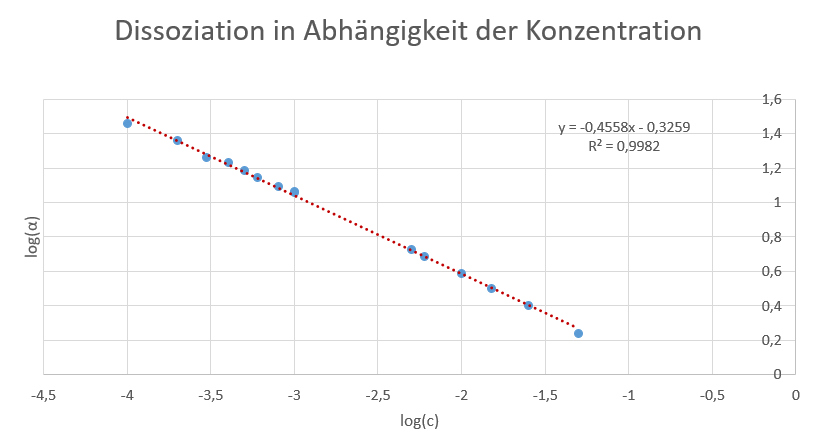
\includegraphics[scale=.7]{../src/img/graph1_40C.png}
    \caption{Bestimmung von $\gamma_\pm$ bei 40$^\circ$C}
\end{figure}

Auch hier nimmt die Dissoziation der Teilchen zu, je geringer die Konzentration ist. Da die Steigungen der beiden Regressionsgeraden annähernd gleich sind,
kann man daraus schließen, dass die Temperatur nur bei entsprechend großen Temperaturunterschieden für die Dissoziation von Bedeutung ist. 



\subsection{Debye-Radius bei 40$^\circ$C}

Zur Berechnung des Debye-Radius wird die entsprächende Molalität für I in Gl. 6 eingesetzt.   

% Table generated by Excel2LaTeX from sheet '40�C'
\begin{table}[H]
  \centering
  \caption{Debye-Radius bei 40$^\circ$}
    \begin{tabular}{lcccc}
    \toprule
    \textbf{Lösung} & \multicolumn{1}{l}{\textbf{Konz [mol/kg]}} & \multicolumn{1}{l}{\textbf{x-Wert: log[c]}} & \multicolumn{1}{l}{\textbf{Debye-Radius [nm] }} & \multicolumn{1}{l}{\textbf{y-Wert: log[rD]}} \\
    \midrule   
    A1    & 50,01 & -1,301 & 44,070 & 1,644 \\
    A2    & 25,01 & -1,602 & 62,325 & 1,795 \\
    A3    & 15,06 & -1,822 & 80,314 & 1,905 \\
    B1    & 10,06 & -1,997 & 98,251 & 1,992 \\
    B2    & 6,05  & -2,218 & 126,734 & 2,103 \\
    A4    & 5,01  & -2,300 & 139,251 & 2,144 \\
    B3    & 1,00  & -2,998 & 311,040 & 2,493 \\
    A5    & 1,00  & -3,001 & 312,130 & 2,494 \\
    C1    & 0,80  & -3,095 & 347,555 & 2,541 \\
    C2    & 0,61  & -3,217 & 400,107 & 2,602 \\
    B4    & 0,51  & -3,297 & 438,566 & 2,642 \\
    C3    & 0,41  & -3,390 & 488,476 & 2,689 \\
    C4    & 0,30  & -3,522 & 568,465 & 2,755 \\
    B5    & 0,20  & -3,698 & 696,063 & 2,843 \\
    C5    & 0,10  & -3,996 & 981,166 & 2,992 \\
    \bottomrule
    \end{tabular}%
  \label{tab:addlabel}%
\end{table}%
 

In Abbildung 4 wird noch mal der logarithmische Zusammenhang grafisch dargestellt..

\begin{figure}[H]
    \centering
    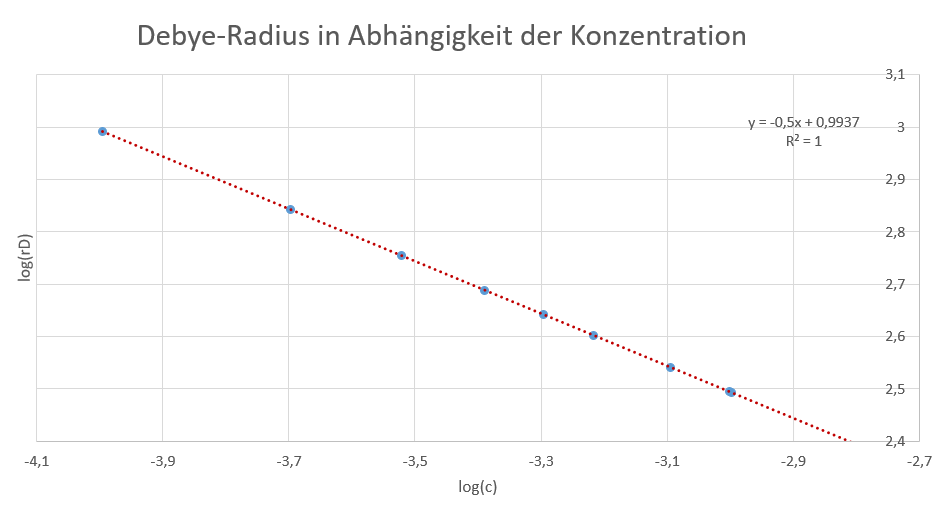
\includegraphics[scale=.7]{../src/img/graph2_40C.png}
    \caption{Debye-Radius bei 40$^\circ$C}
\end{figure}

Wenn man die Geraden von Abbildung 4 und 2 miteinander vergleicht, fällt auf, dass beide mit $m = - 0.5$ exakt die gleiche Steigung haben.
Dies bedeutet, dass bei unserer Versuchsdurchführung die Temperatur im Hinblick auf den Debye-Radius in abhängigkeit der Konzentration
keinen Einfluss hat.
